%%%%%%%%%%%%%%%%%%%%%%%%%%%%%%%%%%%%%%%%%
% Beamer Presentation
% LaTeX Template
% Version 1.0 (10/11/12)
%
% This template has been downloaded from:
% http://www.LaTeXTemplates.com
%
% License:
% CC BY-NC-SA 3.0 (http://creativecommons.org/licenses/by-nc-sa/3.0/)
%
%%%%%%%%%%%%%%%%%%%%%%%%%%%%%%%%%%%%%%%%%

%----------------------------------------------------------------------------------------
%	PACKAGES AND THEMES
%----------------------------------------------------------------------------------------

%\documentclass{beamer}
\documentclass[aspectratio=169]{beamer}
\mode<presentation> {
% The Beamer class comes with a number of default slide themes
% which change the colors and layouts of slides. Below this is a list
% of all the themes, uncomment each in turn to see what they look like.

%\usetheme{default}
%\usetheme{AnnArbor}
%\usetheme{Antibes}
%\usetheme{Bergen}
%\usetheme{Berkeley}
%\usetheme{Berlin} % possivel
%\usetheme{Boadilla}
%\usetheme{CambridgeUS}
%\usetheme{Copenhagen} % possivel
%\usetheme{Darmstadt} % possivel
%\usetheme{Dresden}
%\usetheme{Frankfurt}
%\usetheme{Goettingen}
%\usetheme{Hannover}
%\usetheme{Ilmenau} % possivel
%\usetheme{JuanLesPins} % possivel
%\usetheme{Luebeck}
%\usetheme{Madrid}
%\usetheme{Malmoe}
%\usetheme{Marburg} % possivel
%\usetheme{Montpellier}
%\usetheme{PaloAlto}
%\usetheme{Pittsburgh}
%\usetheme{Rochester}
%\usetheme{Singapore}
%\usetheme{Szeged} % possivel
\usetheme{Warsaw} % igual o que o professor usa

% As well as themes, the Beamer class has a number of color themes
% for any slide theme. Uncomment each of these in turn to see how it
% changes the colors of your current slide theme.

%\usecolortheme{albatross}
%\usecolortheme{beaver} % possivel
%\usecolortheme{beetle} % possivel, pouco contraste
%\usecolortheme{crane}
%\usecolortheme{dolphin} % possivel
%\usecolortheme{dove}
%\usecolortheme{fly}
%\usecolortheme{lily}
%\usecolortheme{orchid}
%\usecolortheme{rose}
%\usecolortheme{seagull} % P&B
%\usecolortheme{seahorse}
%\usecolortheme{whale}
%\usecolortheme{wolverine}

%\setbeamertemplate{footline} % To remove the footer line in all slides uncomment this line
%\setbeamertemplate{footline}[frame number] % To replace the footer line in all
% slides with a simple slide count uncomment this line

 \setbeamertemplate{navigation symbols}{} % To remove the navigation symbols
% from the bottom of all slides uncomment this line
}

\usepackage{graphicx} % Allows including images
\usepackage{booktabs} % Allows the use of \toprule, \midrule and \bottomrule in tables
\usepackage[brazilian]{babel}
\usepackage[utf8]{inputenc}
\usepackage[T1]{fontenc}
\usepackage{animate}
\usepackage{listings}	% Pacote para linguagens
\let\oldlstlistoflistings\lstlistoflistings
 \renewcommand{\lstlistoflistings}{%
   \begingroup%
   \let\oldnumberline\numberline%
   \renewcommand{\numberline}{\lstlistingname~\oldnumberline}%
   \oldlstlistoflistings%
   \endgroup}
   
 \lstdefinelanguage{EMSO}{
  morekeywords={
		Model,FlowSheet,Estimation,Optimization,
		PARAMETERS,VARIABLES,EQUATIONS,DEVICES,SET,SPECIFY,GUESS,CONNECTIONS,
		INITIAL,OPTIONS,ATTRIBUTES,ESTIMATE,EXPERIMENTS,MINIMIZE,MAXIMIZE,FREE,
		Brief,Unit,DisplayUnit,Default,Upper,Lower,Type,final,Valid,Symbol,PosX,PosY,
		Components,LiquidModel,VapourModel,
		Pallete,Icon,Info,Protected,Hidden,
		TimeStep,TimeEnd,TimeUnit,Dynamic,SparseAlgebra,NLPSolver,NLPSolveNLA,NLASolver,DAESolver,
		File,RelativeAccuracy,AbsoluteAccuracy,EventAccuracy,MaxIterations,GuessFile,InitialFile,
		Statistics,Fit,Parameter,Prediction,Significance,BiLateral,RunTests,NumJac,
		using,for,as,to,if,end,else,switch,switchto,when,case,
		in,out,outer, 
		Integer,Real,Boolean,Text,Plugin,Switcher,CalcObject,
		equal,and,or,true,false,
        time,diff,sum,sumt,prod,prodt,transp,min,max,abs,
		sign,round,sinh,cosh,tanh,coth,atan,
		exp,log,ln,sqrt,sin,cos,tan,asin,acos},
  sensitive = true,
  morecomment=[l]{\#},
  morecomment=[s]{\#*}{*\#},
  morestring=[b]",
  morestring=[b]'
}
\lstset{
  basicstyle=\fontfamily{pcr}\fontseries{m}\selectfont\footnotesize,
  commentstyle=\color[rgb]{0,0.5,0}\itshape,
  keywordstyle=\color{blue}\bfseries,
  stringstyle=\color[rgb]{0.5,0,0.5}\itshape,
  showstringspaces=false,
  numbers=left,
  numberstyle=\fontfamily{pcr}\fontseries{m}\selectfont\tiny,
  numberblanklines=false,
  showlines=false,
  belowskip=\bigskipamount{},
  breaklines=true,
  %stepnumber=2,
  tabsize=6,
  %extendedchars=true,
  %float=h,
  frame=tb
}
\renewcommand{\lstlistingname}{Código}
\renewcommand{\lstlistlistingname}{Lista de Códigos}
  
\setbeamercovered{transparent}

\pgfdeclareimage[width=6cm]{logobig}{img/logo/dequi}
\pgfdeclareimage[width=1.0cm]{logo}{img/logo/dequismall}
\logo{\pgfuseimage{logo}}


  

%----------------------------------------------------------------------------------------
%	TITLE PAGE
%----------------------------------------------------------------------------------------

\title[Simulação na Industria Química]{Simulação na Industria Química.\\
Termodinâmica na indústria e em simuladores }
% The short title appears at the bottom of every slide, the full title is only
% on the title page

\author{Eng. Guilherme Braganholo Flôres} % Your name
\institute[PPGEQ - UFRGS] % Your institution as it will appear on the bottom of
% every slide, may be shorthand to save space
{
UNIVERSIDADE FEDERAL DO RIO GRANDE DO SUL \\
ESCOLA DE ENGENHARIA \\
DEPARTAMENTO DE ENGENHARIA QUÍMICA \\
LAB. VIRTUAL DE PREDIÇÃO DE PROPRIEDADE \\ % Your institution for the title page
\medskip
\textit{gbflores89@gmail.com} % Your email address
} 
\date{22 de Outubro de 2015} % Date, can be changed to a custom date

\begin{document}
\logo{\pgfuseimage{logobig}}
\begin{frame}
\titlepage % Print the title page as the first slide
\end{frame}

\begin{frame}
	\frametitle{Guilherme Braganholo Flôres}
	Engenheiro Químico formado pela UFRGS
	\begin{itemize} 
		\item Universidade Federal do Rio Grande do Sul
	\end{itemize}

	Mestrando em Engenharia Química pelo PPGEQ da UFRGS
	\begin{itemize}
		\item Programa de Pós-Graduação em Engenharia Química
	\end{itemize}
 	\pause
	Área de pesquisa:
	\begin{itemize}
		\item LVPP
		\begin{itemize}
			\item Laboratório Virtual de Predição de Propriedades
		\end{itemize}
	\item Modelagem industrial 
	\item Modelos termodinâmicos
	\end{itemize}
\end{frame}


\begin{frame}
\frametitle{Sumário} % Table of contents slide, comment this block out to
% remove it
\tableofcontents % Throughout your presentation, if you choose to use
% \section{} and \subsection{} commands, these will automatically be printed on
% this slide as an overview of your presentation
\end{frame}

%------------------------------------------------------------------------------
%	PRESENTATION SLIDES
%------------------------------------------------------------------------------
\logo{\pgfuseimage{logo}}
\section{Introdução}
\begin{frame}
	\frametitle{O que devemos ter em mente}
	\begin{itemize}
		\item O que é um simulador de processos?
		\item Para que serve um simulador de processo?
		\item Quais são as vantagens do uso de simuladores?
		\item Como são utilizados os simuladores dentro das industrias?
		\item Quais os simuladores disponives? 
		\item Como um simulador funciona?
	\end{itemize}
\end{frame}

\subsection*{Simuladores}

\begin{frame}
	\frametitle{O que são simuladores}
	\begin{columns}[c]
		\column{.5\textwidth}
		\begin{itemize}
			\item Qualquer programa que transforme uma ''coisa'' real 
			em um (ou vários) sistema(s) de equações.
			\note<1>{Simuladores são todos os programas que podemos transformar sistemas
			reais em modelos para “prever o futuro”.\\ .\\
			Por exemplo, os simuladores de carros, simuladores de aviões,
			por que não jogos de carros e aviões (?), simuladores de
			investimento, simuladores empresariais e assim por diante..\\ .\\
			Um exemplo, que mais adiante vocês irão se deparar, é o VPL, uma das simulações
			mais simples que existe, serve para prever como que eu vou pagar um
			investimento, em quanto tempo posso ter o meu dinheiro de volta.}
			\begin{itemize}
				\item <2->O sistema pode ser resolvido por cálculos feitos à
				mão ou programas computacionais
			\end{itemize}
		\end{itemize}
		\note<2>{Outro exemplo extremo são os simuladores de treinamento da NASA,
		muito mais complexos que qualquer simulador de processo, mas o investimento que a NASA fez
		para esses simuladores são pagos pela segurança que eles trazem.\\.\\
		Geralmente o piloto da nave espacial nunca guiou uma de verdade, mas passou horas e horas
		treinando em um simulador, e provavelmente já morreu diversas vezes de forma
		fictícia, é logico.}
		\column{.5\textwidth} % Right column and width
			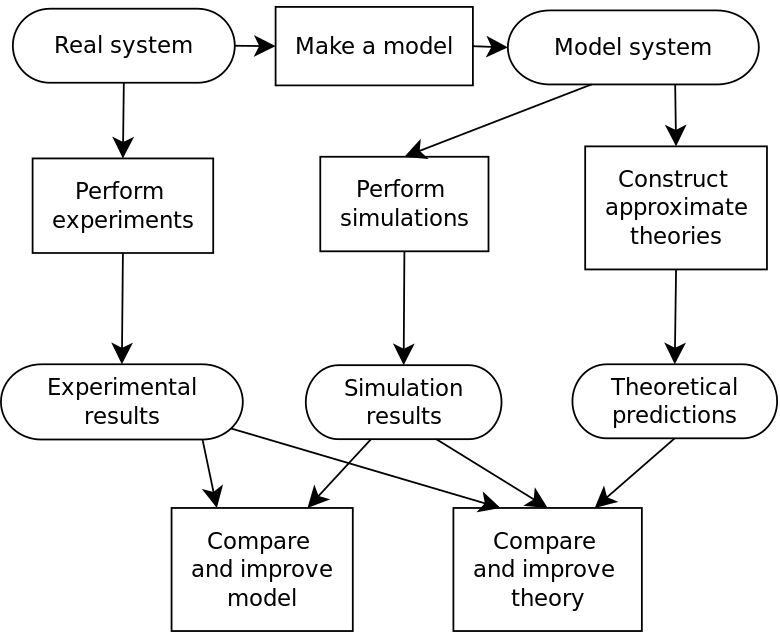
\includegraphics[width=0.95\textwidth]
			{img/Molecular_simulation_process.png}
	\end{columns}
\end{frame}

\begin{frame}
	\frametitle{O que são simulador de processo?}
	\begin{columns}[c] 
		\column{.3\textwidth}
		\begin{itemize}
		  \item Em simuladores de processo a ``coisa'' passa a ser a planta industrial, ou
		parte dela.
		\end{itemize}
		\column{.7\textwidth}
		\begin{center}
			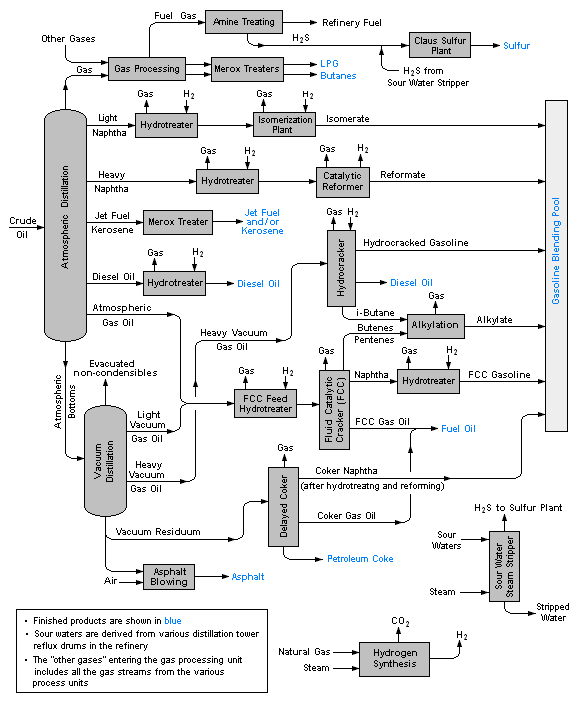
\includegraphics[width=0.5\textwidth]
				{img/RefineryFlow.png}
		\end{center}
	\end{columns}
\end{frame}

\begin{frame}
	\frametitle{Principais motivos para o uso de um simulador}
	Projeto de uma planta química\\
	\note<1>{Quando o cálculo feito à mão é muito custoso, ou seja, podemos dar um
	chute inicial para o cálculo de uma coluna de destilação, por exemplo, mas o
	cálculo rigoroso, será feito apenas via simulador.\\.\\}

	Otimização de uma planta química\\
	\note<1>{Podemos inclusive, otimizar uma planta ainda em estado de
	desenvolvimento.\\.\\}
	
	Fazer diversos experimentos sem custo financeiro ou com custo mínimo!
	\note<1>{E como sabemos, para qualquer otimização, devemos conhecer o
	comportamneto da planta, ou seja, quais são os limites operacionais, e a
	matriz de causa e efeito, se eu mexer neste parâmetro, qual o resultado da
	planta?? e por assim em diante.\\.\\}
	\begin{itemize}
		\item Experimentos que industrialmente são muito demorados podem ser feitos em
		questões de minutos
			\begin{itemize}
				\item Colunas de destilação podem demorar dias para entrar
				em estado estacionário
		\end{itemize}
	\end{itemize}
	\pause
	Segurança
	\begin{itemize}
		\item Pode-se ultrapassar, sem risco os limites operacionais dos equipamentos
	\end{itemize}
\end{frame}


\begin{frame}
	\frametitle{Simuladores mais conhecidos}
	\begin{itemize}
		\item Aspen Technology --> Aspen Plus
		\item Aspen Technology --> Aspen HYSYS
		\item PSE Ltd --> gPROMS
		\item SimSci -->PRO/II \pause 
		\note<1>{Os simuladores mais conhecidos na indústria e na academia são
		estes:\\.\\ O Aspen Plus (caro, mas muito bom) e o Aspen HYSYS... \\
		O HYSYS foi comprado pela Aspen poucos anos atrás e como já era muito
		conhecido, ficou o nome HYSYS, são simuladores de blocos ou seja, coloca os
		equipamentos e o simulador resolve um por vez, até que finalmente o sistema
		inteiro converge.\\.\\
		gPROMS eu sinceramente não conheço, mas sempre ouço falar
		PRO/II segue a mesma linha do Aspen Plus e HYSYS}
		
		\item \textbf{ALSOC Project --> EMSO}
		\item \textbf{VRTech --> iiSE Simulator}
		\note<2>{ E estes dois últimos, o EMSO e o iiSE, são os simuladores que eu
		mais trabalho, a vantagem destes simuladores é que eles são orientados a
		equações, ou seja, transformam o fluxograma de processo em um sistema de
		equações, onde o tamanho do sistema vai variar dependendo da complexidade
		dele.}
	\end{itemize}
\end{frame}

\begin{frame}
	\frametitle{Tipo de simuladores}
	\begin{columns}[t] 
		\column{.5\textwidth}
			\textbf{Simuladores em blocos.}\\
			Aspen Plus, por exemplo.\\
			\begin{itemize}
				\item A simulação é feita por etapas, um bloco por vez.
				\begin{itemize}
					\item Vários sistemas de equações menores resolvidos separadamente
					\item O resultado de um equipamento depende diretamente do 
				equipamento calculado anteriormente.
				\end{itemize}
				\item Apresenta mais problemas com reciclos
			\end{itemize}
		\column{.5\textwidth}
			\textbf{Simuladores orientado a equações.}\\
			EMSO e iiSE, por exemplo.\\
			\begin{itemize}
				\item A simulação é feita em uma unica etapa.
				\begin{itemize}
					\item A simulação inteira é transformado em um unico sistema de equações
					\item A solução dos equipamentos é feita de forma simultanea para
					todos.
				\end{itemize}
			\end{itemize}
	\end{columns}
	\note{Bom, temos dois tipos de simuladores, os simuladores de blocos e os
	orientados a equações\\
	Os simuladores de blocos, como o Aspem, transformam o fluxograma de processo
	em vários sistemas de equações, um para cada equipamento e resolve o
	problema inteiro em etapas.\\.\\
	Por outro lado os simuladores orinetados a equações transformam o fluxograma
	como um todo em um unico sistema de equações e resolve tudo de uma vez só}
\end{frame}

\begin{frame}[plain]
	\frametitle{EMSO}
	\begin{center}
		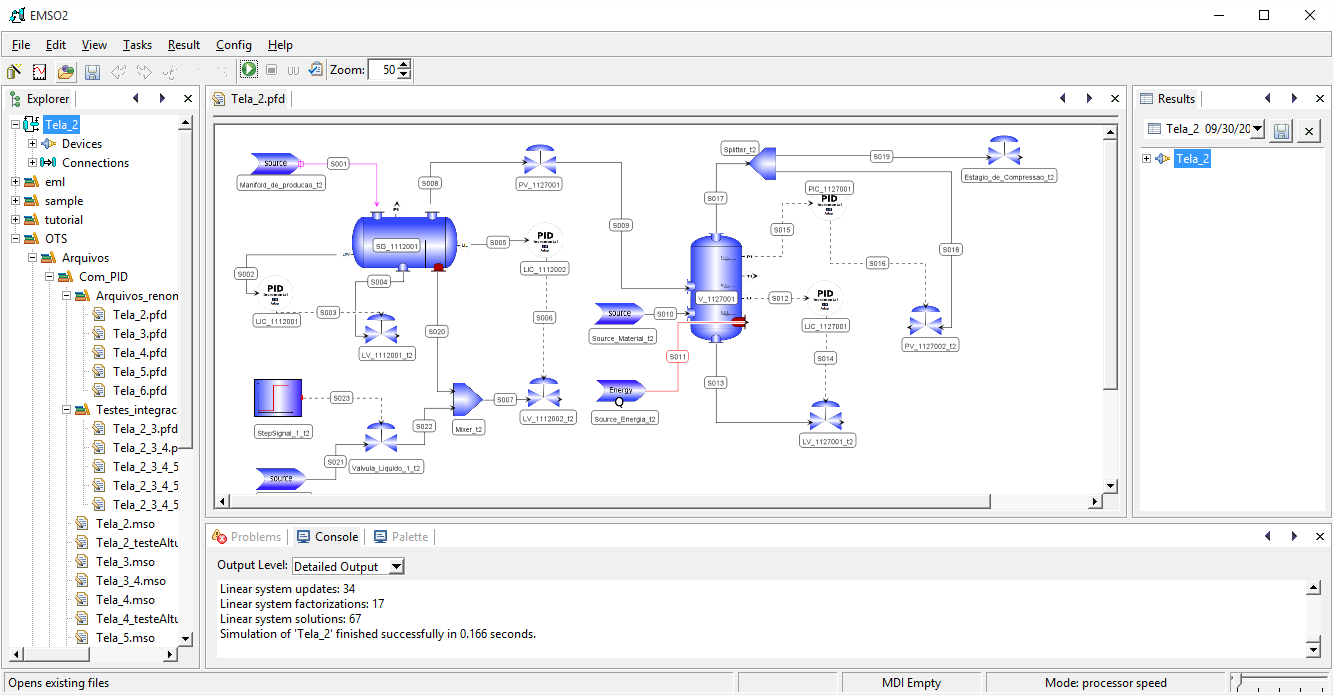
\includegraphics[width=0.9\textwidth]{img/EMSO_1.PNG}
	\end{center}
	\note{Funciona mais ou menos assim, o usuário abre um novo arquivo e vai
	montando a simulação, vai fazendo aos poucos, cada vez que o usuário manda o
	comando para executar a simulação, o simulador automaticamente transforma todos
	os equipamentos (blocos) em um único sistema de equações, pois cada bloco é
	composto por uma serie de equações \\
	No caso este exemplo é um pequeno pedaço de uma plataforma de pertróleo}
\end{frame}

\begin{frame}[plain]
	\frametitle{EMSO}
	\begin{center}
		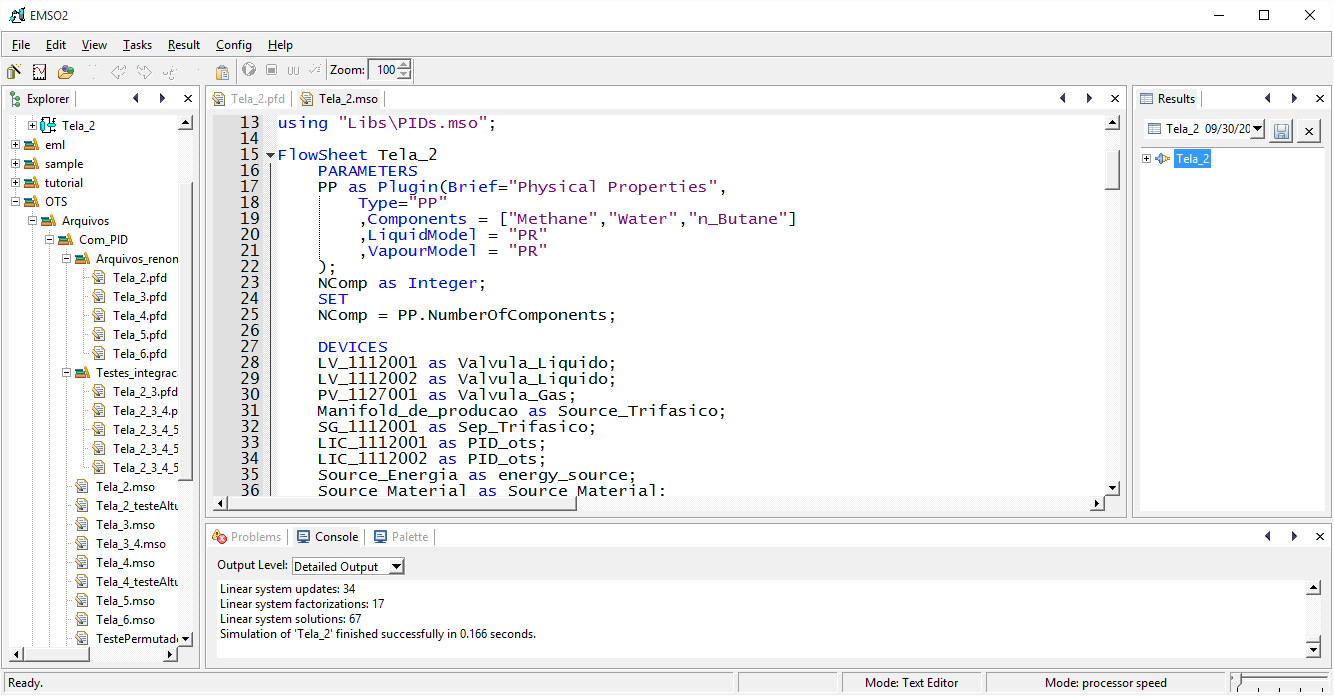
\includegraphics[width=0.9\textwidth]{img/EMSO_2.PNG}
	\end{center}
	\note{Somente depois de tudo transformado em equações, que ai sim o simulador
	começar a calcular o sistema.\\.\\
	Bom ai vai de cada usuário saber o que deseja simular, nesse sentido eu digo
	que da pra simular tudo que acontece na indústria química, desde que utilize o
	simulador adequado }
\end{frame}

\subsection*{Modelos}

\begin{frame}
	Ok já sabemos o que são simuladores, mas como eles funcionam?\\
	\begin{itemize}
	  \item Cada equipamento do simulador é um \code{modelo}
	\end{itemize} \pause
	Como são estes \code{modelos}?
\end{frame}

\begin{frame}[plain]
	\frametitle{Modelo EMSO}
	\footnotesize
		\begin{columns}[t] 
			\column{.5\textwidth}
				 \lstinputlisting[firstline=3, lastline=14, 
				 numbers=none, language=EMSO]
				 {img/pump.mso}
			\column{.5\textwidth}
				 \lstinputlisting[firstline=15, lastline=33, 
				 numbers=none, language=EMSO]
				 {img/pump.mso}
		\end{columns}
	\note{Todos os simuladores tem um código assim implementado, inclusive em
	simuladores de blocos, óbvio que podemos ter implementações mais ou menos
	rigorosas, esse exemplo é uma bomba simplificada, se bem que ainda podemos
	simplificar mais ainda.}
\end{frame}

\begin{frame}[plain]
 	\frametitle{Modelo simplificado}
%  	\framesubtitle{Não façam isso em casa!!}  
	\begin{columns}[c] 
		\column{.5\textwidth}
			 \lstinputlisting[firstline=3, lastline=17, 
			 numbers=none, language=EMSO] 
			 {img/pump2.mso} 
		\note<3>{Por favor, não façam isso em casa, e nem quando estiverem trabalhando
		com um modelo sério\\.\\}
		\pause
		\column{.5\textwidth}
			\begin{itemize}
				\item Por que alguém faz um modelo assim??
				\item Ok mas para que serve um modelo deste tipo??
			\end{itemize}
			\pause
			\begin{block}{}
				\begin{itemize}
					\item Simples, a bomba não é importante na minha simulação, tanto faz se
					esqunta o fluido ou não.
					\item Só preciso dela para um incremento de pressão.
				\end{itemize}
				\note<3>{Isso nos tras outra questão, o quanto certo está o nosso modelo}
			\end{block}
	\end{columns}
\end{frame}


\begin{frame}
	\frametitle{Modelos}
	\begin{columns}[c]
		\column{.3\textwidth}
	\begin{itemize}
	  \item O que eu quero simular? \pause
	  \note<3>{De nada adianta eu criar um modelo se eu não sei o que eu quero
	  fazer com ele, isso é mais ou menos como: Ta indo pra onde? Não sei, mas to
	  indo\\.\\}
	  \item Os modelos estão certos? \pause
	  \note<3>{E agora temos um problema.\\.\\}
	  \begin{itemize}
		\item Não!!!
		\item <alert@3> Todos os modelos estão ``errados''.
	  \end{itemize}
	  \note<3>{O que acontece é que todos os modelos estão errados, não importa o
	  quanto esforço seja empregado para ele, ele vai estar errado. A parte boa da
	  hitória é que mesmo errado, o modelo vai nos ajudar}
	\end{itemize}
		\column{.7\textwidth}
		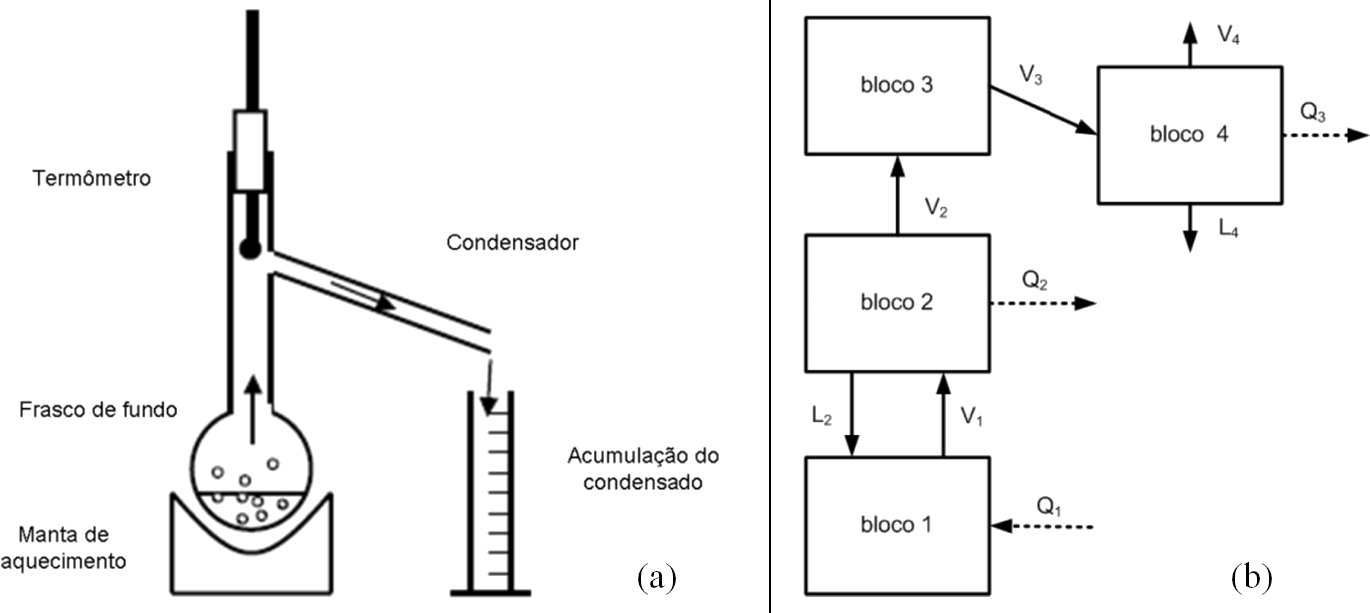
\includegraphics[width=0.9\textwidth]{img/blocos.png}
	\end{columns}
\end{frame}

\begin{frame}
	\frametitle{Confiabilidade dos modelos}
	Mas se todos os modelos estão errados,
	como podemos confiar neles?\\
	\begin{itemize}
	  \item Depende das simplificações que podemos admitir \pause
	  \item Em um modelo rigoroso, por exemplo as simplificações são minimas e
	  tudo que é possivel de ser calculado será calulado!
	\end{itemize}
	\note<2>{Sim os modelos estão errados, mas depende do quanto errado podemos
	admitir, em um modelo simplificado, como eu mostrei anteriormente sabemos que
	foram feitas varias suposições como}
\end{frame}

\begin{frame}
	\frametitle{Confiabilidade dos modelos}
	\begin{columns}[c] 
	\column{.5\textwidth}
		Dependo das simplificações que forem feitas o modelo vai servir para o
		nosso proposito.\\
		\begin{itemize}
			\item Não podemos simplificar no caso de uma bomba, pro exemplo \\
 				\begin{equation*}
				P_{in}=P_{out}
 				\end{equation*}\\
			\pause
			\item Mas em um modelo simplificado podemos desconsiderar a curva da
			bomba
		\end{itemize}
		\column{.5\textwidth}
		\begin{center}
			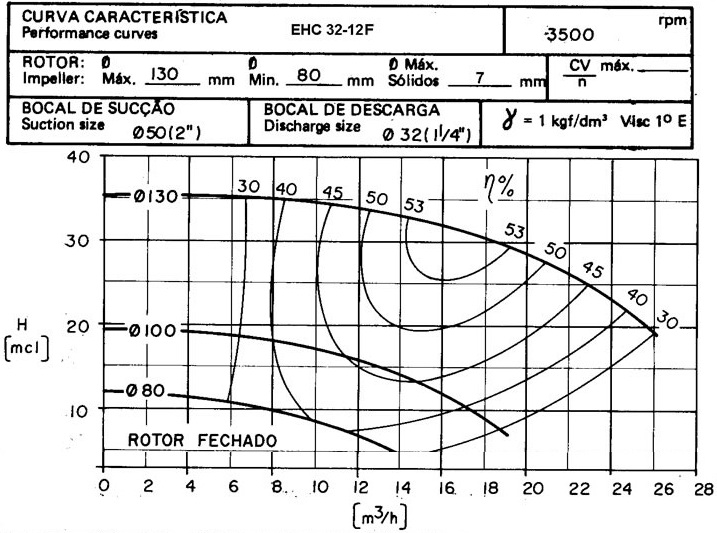
\includegraphics[width=\textwidth]{img/curva_bomba2.jpg}
		\end{center}
	\end{columns}
\end{frame}

\section{Modelos Termodinâmicos}

\begin{frame}
	\frametitle{O que já podemos decidir até o momento?}
	\begin{itemize}
		\item Já definimos o que queremos simular.
		\item Já definimos o simulador.
		\item Já definimos o qunto o nosso modelo pode ser simplificado.
	\end{itemize}
	\pause
	Como calculamos as propriedades termodinâmicas que a simulação irá precisar?
\end{frame}

\begin{frame}
	\frametitle{Tipos de modelos termodinamicos}
	\begin{columns}[t] 
		\column{.5\textwidth}
			\textbf{Componentes puros}\\
			\begin{itemize}
				\item Equacões de estado.
			\end{itemize}
		\column{.5\textwidth}
			\textbf{Misturas}\\
			\begin{itemize}
				\item Equações de estado combinada à regras de misturas.
				\item Modelos de $G^E$ \\ 
				Também conhecidos como modelos de $\gamma$
				\item Modelos de $G^E$ combinado com equações de estado via regra de
				mistura.
			\end{itemize}
	\end{columns}
	\note{Para as substâncias puras, somente podemos utilizar as equações de
	estado, isso porque os modelos de $G^E$ são desenvolvidos para misturas\\.\\
	Todos modelos de $G^E$ são desenvolvidos considerando que o liquido de uma
	substância pura é uma solução ideal, sendo uma solução ideal todos as
	propriedades são do componente puro. \\.\\
	Vamos ver adiante cada classe de modelo}
\end{frame}

\subsection*{Equações de Estado}

\begin{frame}
	\frametitle{Equações de Estado (Equations of State - EOS)}
	\begin{itemize}
		\item De alguma forma relacionam as propriedades $P$, $v$ e $T$ ou
		outras propriedades não mensuráveis
		\item Exemplos: gás ideal, cúbicas (PR, SRK, ...), tipo Virial, SAFT e
		PC-SAFT
		\pause
		\item[]
		\item Partindo de uma EOS e do $Cp^{GI}$ é \textbf{possível calcular todas
		as demais propriedades}: $u$, $h$, $s$, ...
		\item São desenvolvidas para substâncias puras (a maioria)
	\end{itemize}
	\note<1>{São equações para relacionar P, v e T.\\
	O cálculo das demais propriedades é possivel devido as derivações da
	equação de estado e das relações de Maxwell}
\end{frame}

\begin{frame}
	\frametitle{O Gás Ideal}
	É a equação de estado mais comum
	\begin{equation*}
	P=\frac{RT}{v}
	\end{equation*}
	\begin{itemize}
	  \item Baseada nas considerações de que:
	  \begin{enumerate}
	    \item As moléculas do gás não ocupam nenhum volume
	    \item As moléculas do gás não exercem nenhuma força
		intermolecular
	  \end{enumerate}
	\end{itemize}
	Entretanto pode apenas representar a fase gás
\end{frame}

\begin{frame}
	\frametitle{Equações cúbicas - Equação de van der Waals}
	\begin{columns}[c] 
	\column{.6\textwidth}
		\begin{itemize}
		\item Proposta por van der Waals em 1873
		\item Considera as moléculas como esferas \\
		rígidas para representar as forças\\
		repulsivas
		\item Forças de van der Waals descrevem as\\
		forças atrativas
		\item Depende de dois parâmetros: $a$ e $b$
		\end{itemize}
	\column{.3\textwidth}
	\begin{center}
		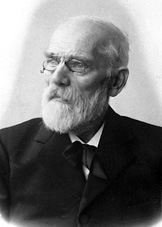
\includegraphics[width=0.8\textwidth]{img/waals.jpg}
	\end{center}
	\end{columns}
	\begin{columns}
		\column{.75\textwidth}
		\begin{footnotesize}
			\begin{exampleblock}{Johannes Diderik van der Waals, Nobel em Física - 1910}
				... for his studies of the physical state of liquids and gases..
			\end{exampleblock}
		\end{footnotesize}
	\end{columns}
\end{frame}

\begin{frame}
	\frametitle{Equações cúbicas - Equação de van der Waals}
	\begin{columns}
		\column{.75\textwidth}
			\begin{exampleblock}{Correção devido ao tamanho das moléculas:}
				volume molar não ocupado pelas moléculas, $v-b$
			\end{exampleblock}
	\end{columns}
	\begin{columns}
		\column{.75\textwidth}
			\begin{exampleblock}{Correção devido às forças intermoleculares
			atrativas:}
			forças atrativas proporcionais a ${}^{1}/{}_{r^6}$ ou
			${}^{1}/{}_{v^2}$
			\end{exampleblock}
	\end{columns}
	\begin{itemize}
		\item Forma final
		\begin{equation*}
		P=\frac{RT}{v-b}-\frac{a}{v^2}
		\end{equation*}
		\item Pode ser re-escrita na forma cúbica como:
		\begin{equation*}
		Pv^3-\left(RT+Pb\right)v^2+av-ab=0
		\end{equation*}
	\end{itemize}
\end{frame}

\begin{frame}
	\frametitle{Equações cúbicas - Equação de van der Waals}
	
	\begin{columns}
		\column{.5\textwidth}
		\begin{itemize}
			\item Os parâmetros $a$ e $b$ da equação de vdW podem ser obtidos a
			partir do ponto crítico: 
		\end{itemize}
			\begin{equation*}
			\left(\frac{\partial P}{\partial v}\right)_{T_r} = \left(\frac{\partial^2
			P}{\partial v^2}\right)_{T_r}=0
			\end{equation*}
			\pause
			\begin{equation*}
			\Downarrow
			\end{equation*}
			\begin{equation*}
			a=\frac{27}{64}\frac{\left(RT_c\right)^2}{P_c} \qquad
			b=\frac{RT_c}{8P_c} 
			\end{equation*}
		
		\column{.5\textwidth}
			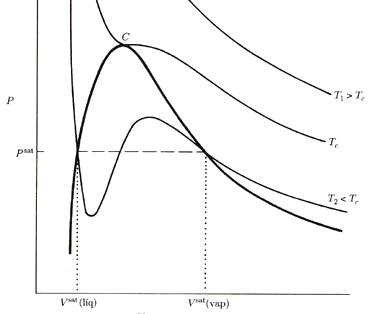
\includegraphics[width=0.8\textwidth]{img/ecuaciones-de-estado.png}
	\end{columns}
	 \note<1>{Ali no ponto ``c'' está a um dos pontos mais importantes para as
	 equações cubicas provenientes da equação de vdW, é o ponto crítico da
	 substância, onde o vapor e o liquíquido assumem as mesmas propriedades.\\.\\
	 Ali também ocorre um ponto de inflexão onde a primeira e a segunda derivadas
	 da equação são zeros.\\.\\
	 Ahh, lembrando que abaixo do ponto crítico, dentro do envelope de faze a
	 curva da equação não tem sentido físico, é apenas uma consequencia matemática}
\end{frame}

\begin{frame}[plain]
	\frametitle{Algumas Equações Cúbicas}
	Outras equações cúbicas:
	\begin{equation*}
		P= \frac{RT}{v-b}-\frac{a(T)}{(v-\epsilon b)(v+\epsilon b)}
	\end{equation*}
	\\
	\begin{equation*}
		a= \frac{\Psi \alpha(T_r) R^2 {T_c}^2}{P_c} \quad b= \Omega \frac{RT_c}{P_c}
		\quad T_r = \frac{T}{T_c} \quad P= \frac{P}{P_c}
	\end{equation*}
	\\
	\begin{table}
		\begin{tabular}{cc|ccccc}
		\hline
		{EoS} & Ano & {$\alpha(T_r)$} & {$\sigma$}& {$\epsilon$}&
		{$\Omega$}& {$\Psi$} \\
		\hline
		vdW  & 1873& $1$ & 0 & 0 & $1/8$ & $27/64$\\
		RK & 1949 & $1/\sqrt{T_r}$ & 1 & 0 & 0.08664& 0.42748\\
		SRK & 1972 & $\alpha_{SRK}$ & 1 & 0 & 0.08664& 0.42748\\
		PR & 1976 & $\alpha_{PR}$ & $1+\sqrt{2}$ & $1-\sqrt{2}$ & 0.07780 & 0.45724\\
		\hline
		\multicolumn{7}{l}{$\alpha_{SRK}=\left[1+\left(0.48+1.574w-0.176w^2\right)
		\left(1-\sqrt{T_r}\right) \right]^2$}\\
		\multicolumn{7}{l}{$\alpha_{PR}=\left[1+\left(0.37464+1.54226w-0.2699w^2\right)
		\left(1-\sqrt{T_r}\right) \right]^2$}\\
		\hline
		\end{tabular}
	\end{table}
	\note{Aqui estão algumas modificações da equação de vdW, e pode ser escrita de
	uma forma genérica, o que é estremamente util pois podemos encontrar as
	propriedades em função dos parâmetros ou seja, derivamos apenas uma vez}
\end{frame}

\begin{frame}
	\frametitle{Comportamento $PvT$ de acetonitrila calculado com PR}
	\begin{center}
		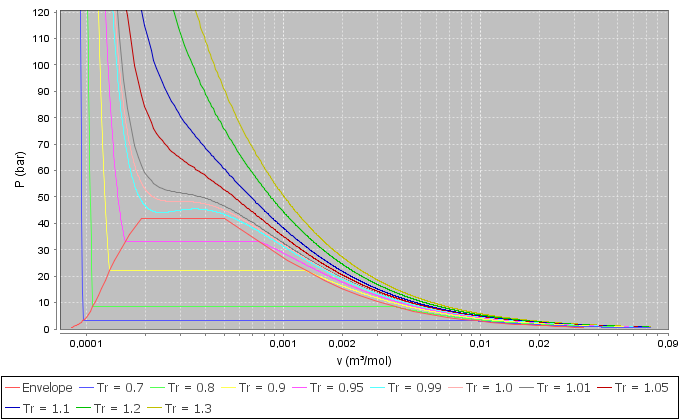
\includegraphics[width=0.7\textwidth]{img/Acetonitrila.png} 
	\end{center}
\end{frame}

\subsection*{Regras de Mistura}

\begin{frame}
	\frametitle{Regras de Mistura}
	\begin{columns}[c]
	\column{.5\textwidth}
		\begin{itemize}
			\item A grande maioria das equações de estado são desenvolvidas para
			\textbf{substâncias puras}!
			\item Para misturarmos substâncias devemos utilizar \textbf{regras de
			misturas}
			\pause
			\begin{itemize}
				\item Regras de misturas combinam as propriedades das substâncias puras em
				um único parâmetro para que possamos utilizar nas EoS	
			\end{itemize}
		\end{itemize}
	\column{.5\textwidth}
		\pause
		\begin{itemize}
			\item A primeira regra de mistura veio pela necessidade da primeira EoS
			\begin{block}{Regra de mistura de van der Waals}
			\begin{equation*}
			a = \sum_i\sum_j{y_iy_ja_{ij}}(1-k_{ij}) \quad a_{ij}= \sqrt{a_i a_j}
			\end{equation*}
			\begin{equation*}
			b = \sum_i{b_iy_i}
			\end{equation*}
			\end{block}
		\end{itemize}
	\end{columns}
	
	\note<1>{Então, temos como calcular os componentes puro, mas sabemos que na
	industria não encontramos apenas componentes puros, e como podemos fazer para
	mistura-los?\\.\\
	Como vdW é um cara inteligente e sabia que deveria servir para misturas
	também, ele decidiu combinar os parâmetros das equações, assim surgiu a
	primeira regra de mistura, uma das mais simples que encontramos na literatura}
\end{frame}

\begin{frame} 
	\frametitle{Outras regras de mistura}
		\begin{columns}[c]
	\column{.7\textwidth}
	Algumas regras de misturas mais complexas
	\begin{itemize}
		\item Huron–Vidal mixing rule (MHV)(1990)
		\item Predictive Soave-Redlich-Kwon Model (PSRK) (1991)
		\item Universal Mixing Rule (UMR) (2004)
		\item Universal and Generic Mixing Rule (UGMR)(2010)
		\item A Self-Consistent Mixing Rule (SCMR)(2012)
	\end{itemize}
	\column{.35\textwidth}
			\begin{block}{Huron–Vidal mixing rule}
			\begin{equation*}
			a = b \left[ \sum  x_i \left(\frac{a_i}{b_i} \right) + \frac{G^E}{C^*}
			\right] 
			\end{equation*}
			\begin{equation*}
			b = \sum_i{b_iy_i}
			\end{equation*}
			\end{block}
	\end{columns}
	\note{Entretanto, posteriormente apareceram regras de misturas mais
	elaborada em que foram introduzidos um parâmetro $k_{ij}$ para melhorar
	o resultado comparando com os dados experimentais.\\.\\
	Quando foi introduzido esse parâmetro binário $k_{ij}$ ajustado também tiveram
	a idéia de substituir os parâmetros de interação por um modelo de coeficiente
	de atividade (modelos de $G^E$) }
\end{frame}

\subsection*{Equilíbrio de fases}

\begin{frame}
	\frametitle{Modelos de $G^E$}
	\begin{columns}[c]
		\column{.4\textwidth}
		Também conhecidos como:
		\begin{itemize}
			\item Modelos de coeficiente de atividade (da fase líquida)
			\begin{itemize}
				\item Modelos de $\gamma$
			\end{itemize}
		\end{itemize}
		São modelos para representar a não idealidade da fase líquida
		\begin{itemize}
			\item Em sua principal formulação considera o vapor como \\
			\textbf{gás ideal}
		\end{itemize}
		\column{.6\textwidth}
		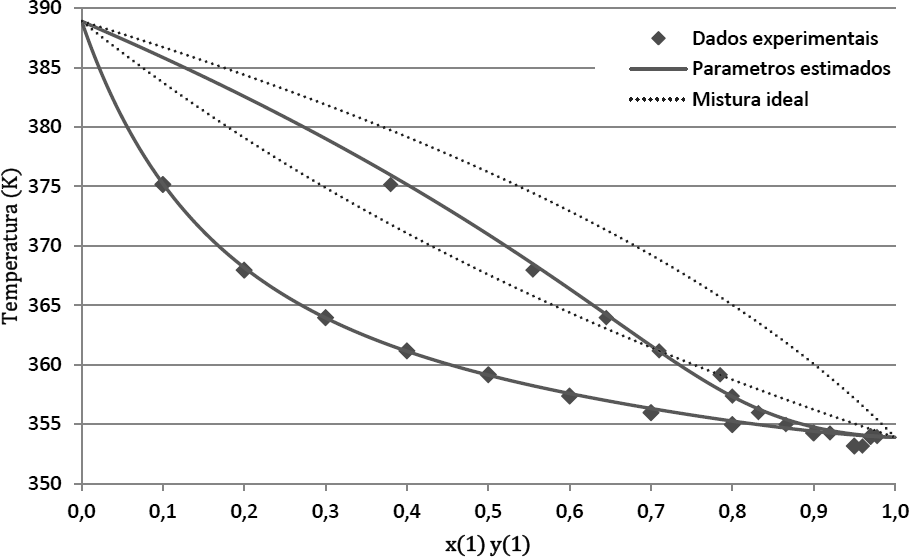
\includegraphics[width=1.0\textwidth]{img/VLE_ideal.png}
	\end{columns}
\end{frame}

\begin{frame}
	\frametitle{Lei de Raoult (Solução ideal)}
		\begin{columns}[c]
		\column{.4\textwidth}
			A Lei de Raoult considera a fase líquida como ideal, com esta preposição temos
			$\gamma = 1$
		\begin{equation*}
		P y_i = x_i P_i^{sat}
		\end{equation*}
		\column{.6\textwidth}
			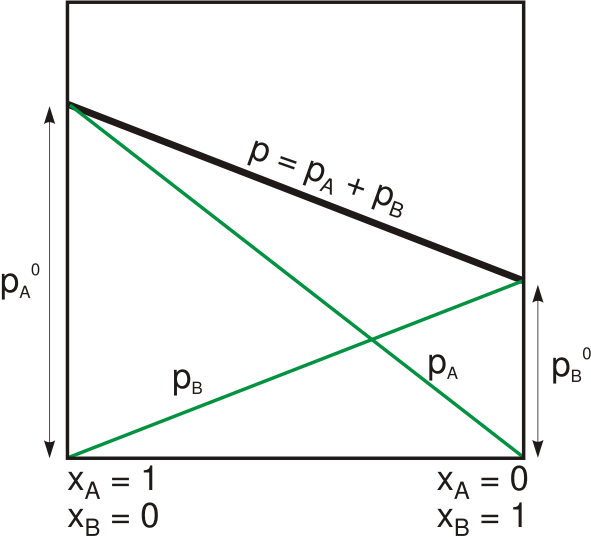
\includegraphics[width=0.8\textwidth]{img/Raoultov_zakon.png}
	\end{columns}
	\note{A Lei de Raout na verdade nem deveria estar aqui, pois ela considera o
	liquido como uma solução ideal.\\.\\
	Entretanto em misturas mais complexas não podemos usar a lei de raout}
\end{frame}

\begin{frame}
	\frametitle{Lei de Raoult modificada}
	Entetanto sabemos que são apenas casos raros que podemos considerar a fase
	líquida como ideal.
	\begin{itemize}
		\item Mistura de n-hexano (\ce{C6H14}) + n-heptano
		(\ce{C7H16}) por exemplo é possível de assumirmos como ideal
		\item Mitura de n-hexano (\ce{C6H14}) + n-dodecano (\ce{C12H26}) já não é
		mais possivel de assumir como ideal.
	\end{itemize}
	\pause
		\begin{equation*}
		P y_i = x_i \gamma_i P_i^{sat}
		\end{equation*}
	\note<1>{Então, em casos não ideais, não podemos mais utilizar a lei de
	Raoult, que é muito limitada. Devemos utilizar a Lei de Raout Modificada, o
	que entre aspas é só colocar aquele $\gamma$ ali, mas já vou mostrar o
	desenvolvimento para vocês}
\end{frame}

\begin{frame}
	\frametitle{Equilíbrio Líquido - Vapor}
	\begin{columns}
	\column{.5\textwidth}
	
	\begin{itemize}
		\item Equilíbrio Mecânico, $P^l=P^v$
		\item Equilíbrio Térmico, $T^l=T^v$
		\item Equilíbrio Químico, $\mu_i^l=\mu_i^v$
	\end{itemize}
	\end{columns}
\end{frame}

\begin{frame}
	\frametitle{Equilíbrio Líquido - Vapor}
	\begin{itemize}
		\item No equilíbrio, $\mu_i^l=\mu_i^v$ o que implica em
		$\hat{f}_i^l=\hat{f}_i^v$
		\item que, com a definição de coefciente de fugacidade para ambas
		as fases, se torna:
		\begin{equation*}
		P y_i \hat{\phi}_i^v = P x_i \hat{\phi}_i^l
		\end{equation*}
		\item e consequentemente:
		\begin{equation*}
		y_i \hat{\phi}_i^v = x_i \hat{\phi}_i^l
		\end{equation*}
		\item Para uma substância pura:
		\begin{equation*}
		\phi_i^v =\phi_i^l =\phi_i^{sat}
		\end{equation*}
	\end{itemize}
\end{frame}

\begin{frame}
	\frametitle{Equilíbrio Líquido - Vapor}
	\begin{itemize}
		\item Utilizando o coeficiente de fugacidade para a fase vapor e
		coeficiente de atividade para a fase líquida, a igualdade de
		fugacidade se torna:
		\begin{equation*}
		P y_i \hat{\phi}_i^v = x_i \gamma_i f_i
		\end{equation*}
		\item Para baixas pressões usualmente assumimos um vapor se
		comportando como gás ideal e que $f_i \cong P_i^{sat}$:
		\begin{equation*}
		P y_i = x_i \gamma_i P_i^{sat}
		\end{equation*}
	\end{itemize}
\end{frame}

\begin{frame}
	\frametitle{Equilíbrio Líquido - Vapor}
	\begin{itemize}
		\item Utilizando o coeficiente de fugacidade para a fase vapor e
		coeficiente de atividade para a fase líquida, a igualdade de
		fugacidade se torna:
		\begin{equation*}
		P y_i \hat{\phi}_i^v = x_i \gamma_i f_i
		\end{equation*}
		\item Para baixas pressões usualmente assumimos um vapor se
		comportando como gás ideal e que $f_i \cong P_i^{sat}$:
		\begin{equation*}
		P y_i = x_i \gamma_i P_i^{sat}
		\end{equation*}
	\end{itemize}
	\note{Agora com o Lei de Raout desenvolvida, ali no lugar do $\gamma_i$ que
	colocaremos o resultado do modelo de $\gamma$}
\end{frame}

\section{Modelos de $G^E$}

\begin{frame}
	\frametitle{Modelos de $G^E$}
	\begin{columns}
		\column{.5\textwidth}
		Modelos Ajustados
		\begin{itemize}
			\item Não preditivos
			\item Muitos parâmetros
			\item Melhores resultados
		\end{itemize}

		\column{.5\textwidth}
		Modelos ``Teóricos''
		\begin{itemize}
			\item Preditivos
			\item Número de parâmetros consideravelmente menor
			\item Melhor embasamento teórico
		\end{itemize}
	\end{columns}
\end{frame}



\subsection*{Modelos ajustados}

\begin{frame}
	\frametitle{Modelos de $G^E$ ajustados a dados experimentais}
	\begin{itemize}
		\item São modelos com pouca fundamentação teórica
		\item Modelos que dependem de parâmetros binários
		\begin{itemize}
			\item Cada par de substâncias tem um conjunto de parâmetros
		\end{itemize}
	\end{itemize}
	\note{São modelos geralmente mais simples, e por serem ajustados, geralmente
	produzem resultados melhores.\\.\\
	São modelos muito utilizados quando se quer ver o comportamento de uma mstura
	espessifica e já estão disponiveis os parâmetros. O grande problema destes
	modelos é que para cada par de substâncias é necessário um conjunto de
	parâmetros.}
\end{frame}


\begin{frame}
	\frametitle{Margules}
	Para uma mistura binária
		\begin{equation*}
		\left\{\begin{matrix}
		\ln \gamma_1 = \left [ A_{12}+2 \left(A_{21}-A_{12} \right)x_1 \right]x_2^2
		\\ 
		\\
		\ln \gamma_2 = \left [ A_{21}+2 \left(A_{12}-A_{21} \right)x_2 \right]x_1^2
		\end{matrix}\right.
		\end{equation*}
		\pause
		Se $A_{12} = A_{21} = A$
		\begin{equation*}
		\left\{\begin{matrix}
		\ln \gamma_1 = Ax_2^2
		\\ \\
		\ln \gamma_2 = Ax_1^2
		\end{matrix}\right.
		\end{equation*}
		\note<1>{Um modelo bastante simples e bem didático é o modelo de margules de
		dois parâmetros, simples, e rápido para calcular em aula, bom para
		demosntração entretanto não aceita misturas com grande não idealidade, o que
		para a industria já não é algo tão desejavel.\\.\\
		Uma simplificação que pode ser feita para sistemas simétricos é o modelo de
		margules de um parâmetro}
\end{frame}

\begin{frame}
	\frametitle{NRTL (Non-Random Two-Liquid)}
	Para uma mistura binária
		\begin{equation*}
		\left\{\begin{matrix}
		\ln \gamma_1 = x_2^2 \left [\tau_{21} \left ( \frac{G{21}}{x_1+x_2G_{21}}
		\right )^2 + \frac{\tau_{12} G_{12}}{\left ( x_2+x_1 G_{12} \right )^2}\right]
		\\ 
		\\
		\ln \gamma_2 = x_1^2 \left [\tau_{12} \left ( \frac{G{12}}{x_2+x_1G_{12}}
		\right )^2 + \frac{\tau_{21} G_{21}}{\left ( x_1+x_2 G_{21} \right )^2}\right]
		\end{matrix}\right.
		\end{equation*}
		Sendo
		\begin{equation*}
		\left\{\begin{matrix}
		\ln G_{12} = -\alpha_{12}\tau_{12}
		\\ \\
		\ln G_{21} = -\alpha_{21}\tau_{21}
		\end{matrix}\right.
		\quad
		\textup{e}
		\quad
		\left\{\begin{matrix}
		\ln \tau_{12} = \frac{\Delta g_{12}}{RT}
		\\ \\
		\ln \tau_{21} = \frac{\Delta g_{21}}{RT}
		\end{matrix}\right.
		\end{equation*}
		\note{Dos modelos um dos de maior aplicação é o NRTL, um modelo já melhor
		elaborado e digamos para a tecnolgia de hoje, até fácil de ser calculado à
		mão em um sistema binário.\\.\\
		É um modelo que já aceita o equilíbrio líquido líquido, e faz tudo que é tipo
		de cálculo líquido vapor.\\.\\
		Agora calcular ele para uma mistura de 3 substâncias já é algo mais
		trabalhoso, principalemnte se pegar a forma mais rigorosa do modelo.\\.\\
		E novamente, para cada par de substâncias é necessário uma matriz de
		parâmetros diferente}
\end{frame}

\begin{frame}
	\frametitle{NRTL (Non-Random Two-Liquid)}
	Para a mistura multicomponente
		\begin{equation*}
			\ln{\gamma_i} = \frac{\sum_{j=1}^n{x_j \tau_{ji} G_{ji} }}
				{\sum_{k=1}^n{x_k G_{ki} }} +
			\sum_{j=1}^n\frac{x_j G_ij}{\sum_{k=1}^n x_k G_{kj}}
			\left ( \tau_{ij}- \frac{\sum_{m=1}^n x_m \tau_{mj} G_{mj} }
			{\sum_{k=1}^n{x_k G_{kj} }} \right )
		\end{equation*}
		\\
		\begin{equation*}
			G_{ij} = \exp \left ( -\alpha_{ij}\tau_{ij} \right )
		\end{equation*}
		\\
		\begin{equation*}
			\alpha_{ij} = \alpha_{ij0} + \alpha_{ij1}T
		\end{equation*}
		\\
		\begin{equation*}
			\tau_{ij} = A_{ij} + \frac{B_{ij}}{T} + \frac{C_{ij}}{T^2} +D_{ij}\ln T
			+E_{ij}T^{F_{ij}}
		\end{equation*}
\end{frame}

\subsection*{Modelos teóricos}

\begin{frame}
	\frametitle{Modelos de $G^E$ com melhor embasamento teórico}
	\begin{columns}[c]
		\column{.3\textwidth}
		\begin{itemize}
		  	\item UNIQUAC
			\item UNIFAC
			\item PSRK
			\item COSMO-SAC
			\item COSMO-RS
			\item F-SAC
		\end{itemize}
		\pause
		\column{.4\textwidth}
		\begin{block}{}
			\begin{equation*}
				\ln{\gamma_i} = \ln{\gamma_i^{comb}} + \ln{\gamma_i^{res}}
			\end{equation*}
		\end{block}
			
	\end{columns}
	
	\note<1>{Agora os modelos como daria para dizer ``mais teóricos'', dá para
	calcular a mão? olha até da, o UNIQUAC vai com um certo grau de paciência mas
	é sempre prefirivel um computador.\\.\\
	Uma coisa interessante é que estes modelos trabalham com duas contribuições.
	uma combinatorial (forma e tamanho) e uma residual (interação binária)}
\end{frame}

\begin{frame}
	\frametitle{UNIQUAC (UNIversal QUAsiChemical)}
		\begin{columns}[t]
		\column{.4\textwidth}
			\begin{block}{}
				\begin{equation*}
					\ln{\gamma_i} = \ln{\gamma_i^{comb}} + \ln{\gamma_i^{res}}
				\end{equation*}
			\end{block}
			\begin{itemize}
				\item [$r_i$] molécula pura
				\item [$q_i$] molécula pura
				\item [$\tau_{ij}$] interação binária
				\begin{itemize}
					\item Um conjunto para cada par de substâncias
				\end{itemize}
			\end{itemize}
		
		\column{.7\textwidth}
		\begin{equation*}
			\ln{\gamma_i^{comb}} = \left(1-V_i+\ln V_i \right)
			- \frac{z}{2}q_i \left(1- \frac{V_i}{F_i} + \ln{\frac{V_i}{F_i}} \right)
		\end{equation*}
		\begin{equation*}
			V_i = \frac{r_i}{\sum_j r_j x_j} \qquad F_i = \frac{q_i}{\sum_j q_j x_j}
		\end{equation*}
		\noindent\rule{\textwidth}{0.1pt}
		\begin{equation*}
			\ln{\gamma_i^{res}} = q_i \left(1- \ln{\frac{\sum_j q_j x_j \tau_{ji}}{\sum_j
			q_j x_j}} - \sum_j{\frac{q_j x_j \tau_{ij}}{\sum_k q_k x_k \tau_{kj}}}
			\right)
		\end{equation*}
		\begin{equation*}
			\tau_{ij} = e^{\frac{-\Delta u_{ij}}{RT}}
		\end{equation*}
	\end{columns}
	\note{O UNIQUAC é um modelo muito mais elaborado, ele já utiliza parâmetros
	das moléculas puras, como o $r_i$ e o $q_i$ entretanto os parâmetros de
	interação continuam sendo ajustados para cada par de moléculas}
\end{frame}


\begin{frame}
	\frametitle{UNIFAC~(Do) -- Contribuição de Grupos}
	\begin{columns}[t]
		\column{.4\textwidth}
			\begin{center}
				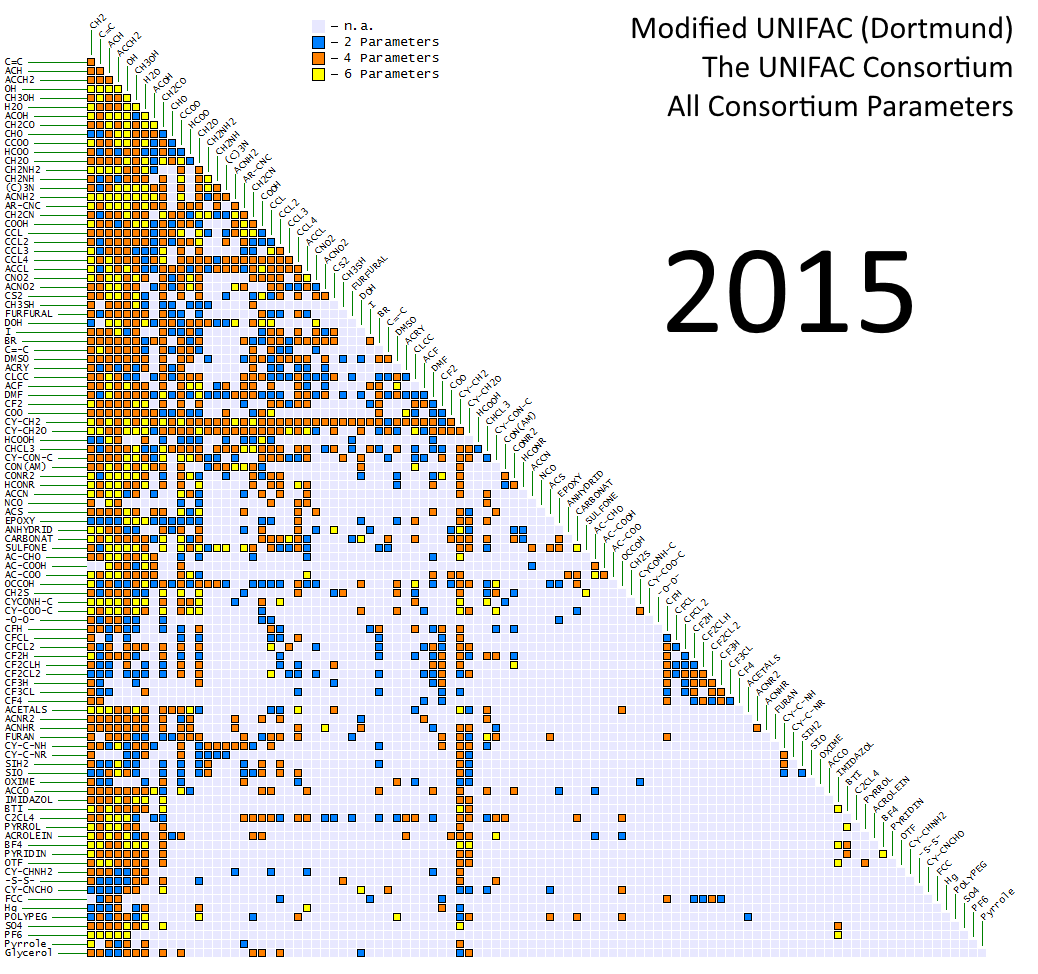
\includegraphics[width=\textwidth]{img/UNIFACDO_2015.png}
			\end{center}
		\column{.6\textwidth}
			\begin{itemize}
				\item Parte do mesmo equacionamento do modelo UNIQUAC
				\item As moléculas agora são grupos funcionais
				\begin{itemize}
					\item \ce{CH3}, \ce{CH2}, \ce{CH}, \ce{CH}
					\item \ce{H2O} (água)
					\item \ce{OH} (álcool)
					\item \ce{ACH}, \ce{AC} (aromático)
					\item \ce{CH3NH2} (amina primária)
				\end{itemize}
				\item A interação binária é entre os grupos
			\end{itemize}
	\end{columns}
	\note{O modelo UNIFAC é uma derivação do modelo UNIQUAC, o seu equacionamento
	é basicamente o mesmo, entretanto passa a não utilizar as moléculas como
	parâmetros e sim um grupo fuincional.\\.\\
	Com a implementação dos grupos funcionais o modelo ganhou a capacidade
	preditiva, ou seja, não é necessário o o ajuste para cada molécula}
\end{frame}

\begin{frame}
	\frametitle{COSMO-RS -- Teoria de superfície de contato}
	\begin{columns}[c]
		\column{.3\textwidth}
			\begin{center}
				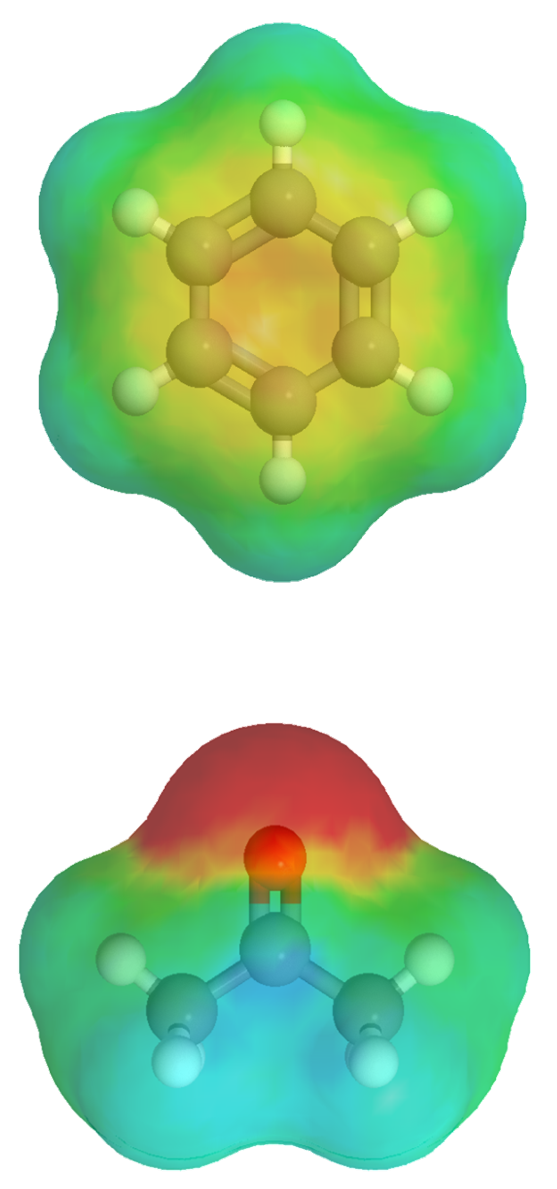
\includegraphics[width=0.65\textwidth]{img/contato1}
			\end{center}

		\column{.7\textwidth}
		\begin{itemize}
			\item Primeiramente aplica-se a técnica COSMO Klamt (1993) para cada
			molécula isolada
			\item São determinadas as cargas aparentes induzidas pela molécula em uma
			\emph{cavidade} \pause
			\item Várias aproximações são assumidas nesta etapa:
			\begin{itemize}
			\item Cavidade formada por esferas de raios fixos envolvendo os átomos
			\item Imersa em um condutor perfeito
			%\item Métodos utilizados nos cálculos: AM1, RM1, DFT, MP2, etc.
			\item Correções para os elétrons fora da cavidade
			\item \ldots
		\end{itemize}
		\end{itemize}
	\end{columns}
	\note<1>{Agora o modelo não utiliza mais contribuição de grupos e toda a parte
	combinatorial é referente a molécula inteira, assim como o termo residual,
	entretanto continua sendo um modelo preditivo pois os parâmetros são
	calculados pelo metodo COSMO, que utiliza termodinâmica estatistica e calculos
	quanticos.\\.\\
	Métodos utilizados nos cálculos: AM1, RM1, DFT, MP2, etc.}
\end{frame}

\begin{frame}
\frametitle{COSMO-RS -- Teoria de superfície de contato}
\begin{columns}[c]
\column{.3\textwidth}
\begin{center}
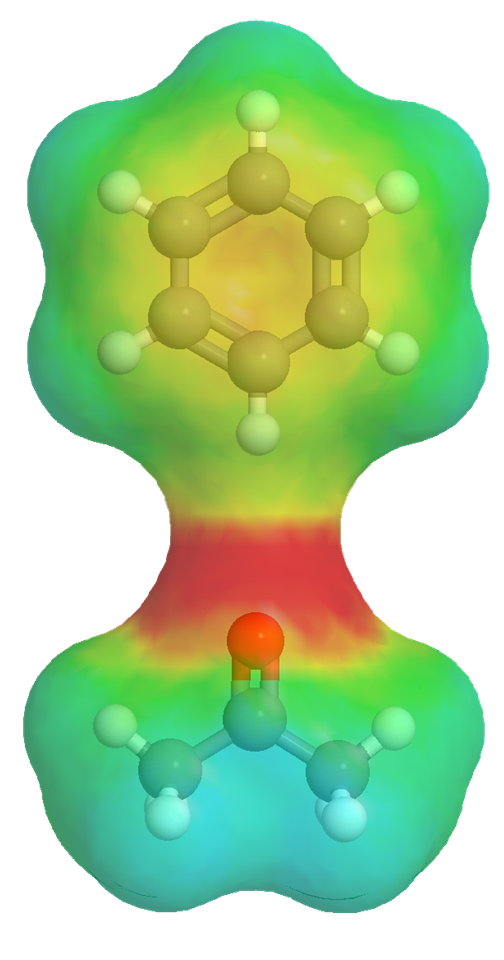
\includegraphics[width=0.7\textwidth]{img/contato2}
\end{center}
\column{.7\textwidth}
\begin{itemize}
    \item Na teoria de superfícies de contato presente no COSMO-RS Klamt 1995,
    	as moléculas são colocadas sequencialmente em contato \pause
    \item A cada contato entre moléculas, o condutor é parcialmente excluído
    \item Se as moléculas forem totalmente circundadas por outras moléculas, a solução \emph{real} seria obtida
\end{itemize}
\end{columns}
\end{frame}

\begin{frame}
\frametitle{Perfil sigma -- $p(\sigma)$}
\begin{columns}[c]
\column{.6\textwidth}
\begin{center}
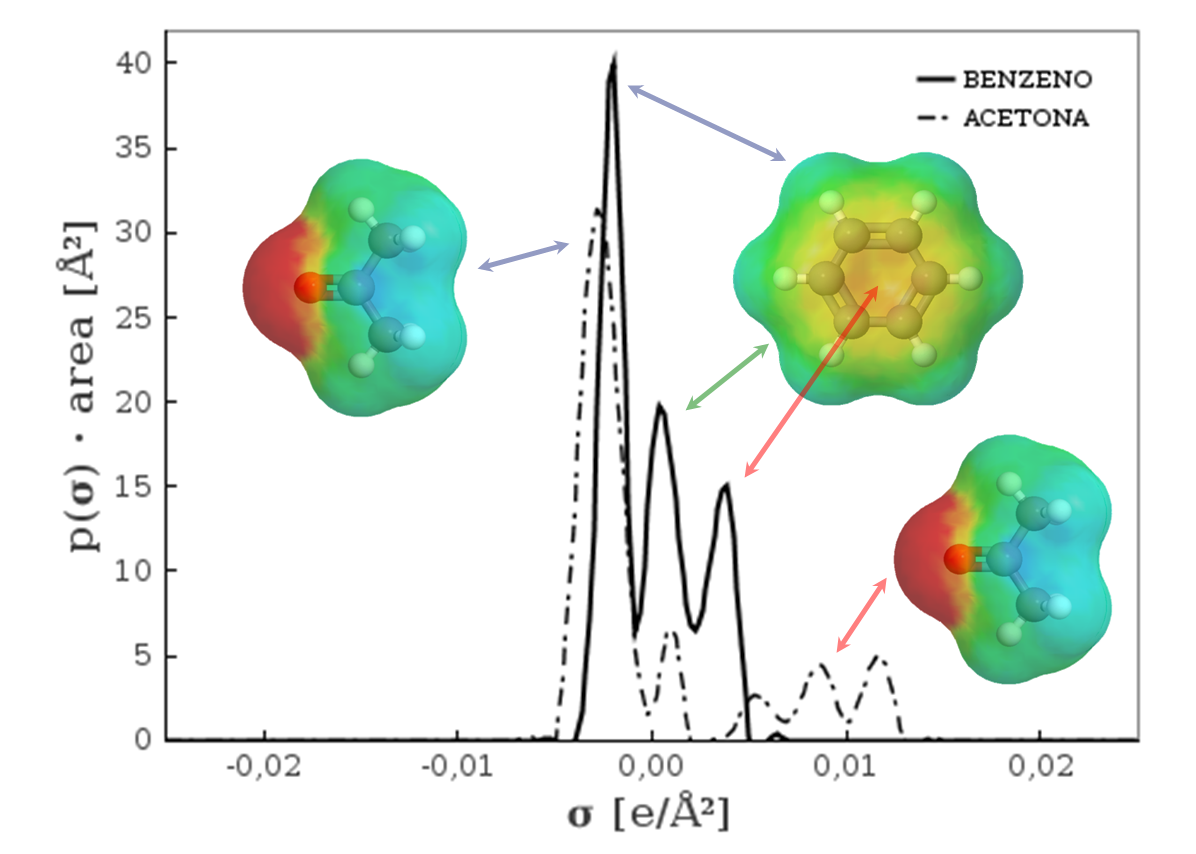
\includegraphics[width=0.8\textwidth]{img/perfilsigma}
\end{center}
\column{.5\textwidth}
\begin{itemize}
    \item Para o tratamento de termodinâmica estatística,
    	a distribuição 3D de cargas aparentes é projetada em um histograma
    \item Esta distribuição de probabilidades é então utilizada para
    	calcular as interações de substâncias em mistura
\end{itemize}
\end{columns}
\pause
\scriptsize
\begin{itemize}
\item É sempre \textbf{desejável} expressar as propriedades de uma solução
em termos que podem ser calculados completamente a partir das propriedades dos
componentes puros -- Prausnitz (1999).
\end{itemize}
\end{frame}

\begin{frame}
	\frametitle{Programa JCOSMO: perfil sigma de substâncias puras}
	\begin{columns}[t]
		\column{.65\textwidth}
		\begin{center}
			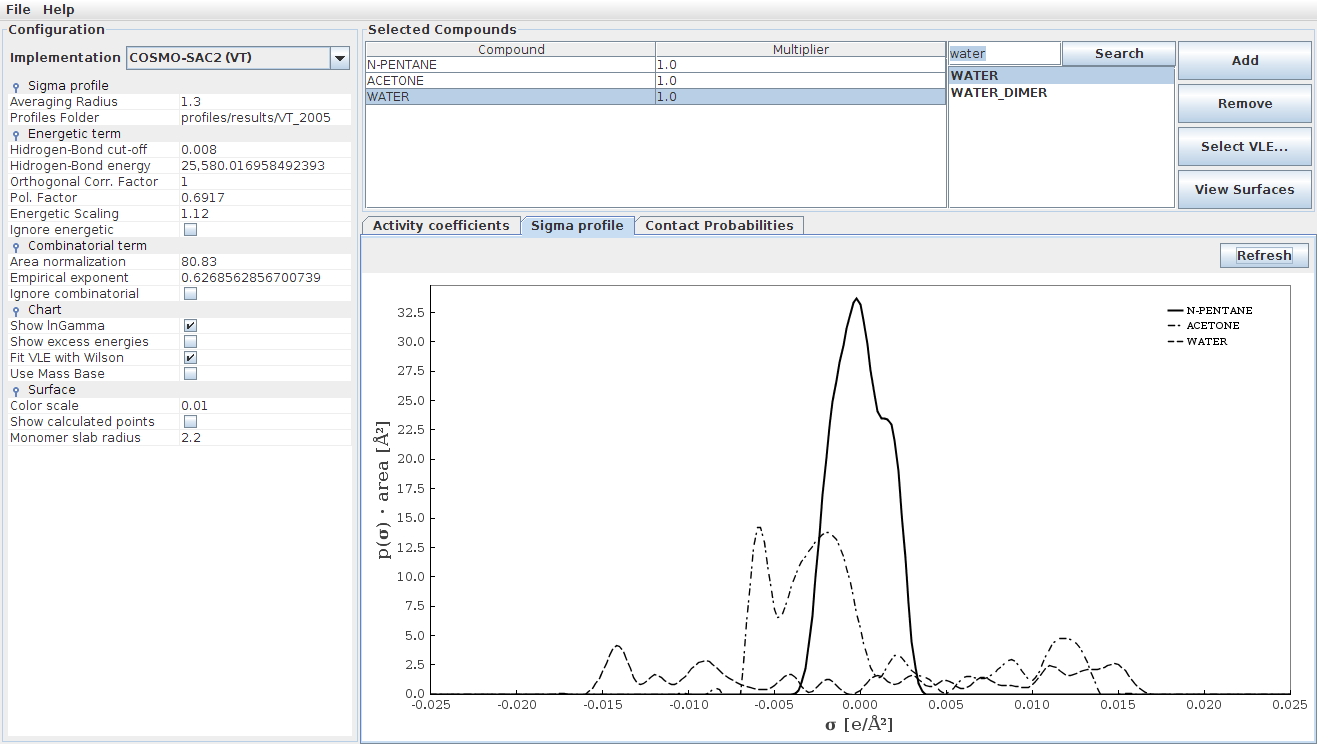
\includegraphics[width=1\textwidth]{img/jcosmoPerfilSigma}
		\end{center}
	
		\column{.3\textwidth}
		\begin{center}
			
\includegraphics[width=1\textwidth]{img/jcosmo_qr}
		\end{center}
	\end{columns}
\end{frame}
 

\begin{frame}
  \frametitle{Programa JCOSMO: cálculos de coef. de atividade e VLE}
	\begin{columns}[t]
		\column{.6\textwidth}
		\begin{center}
			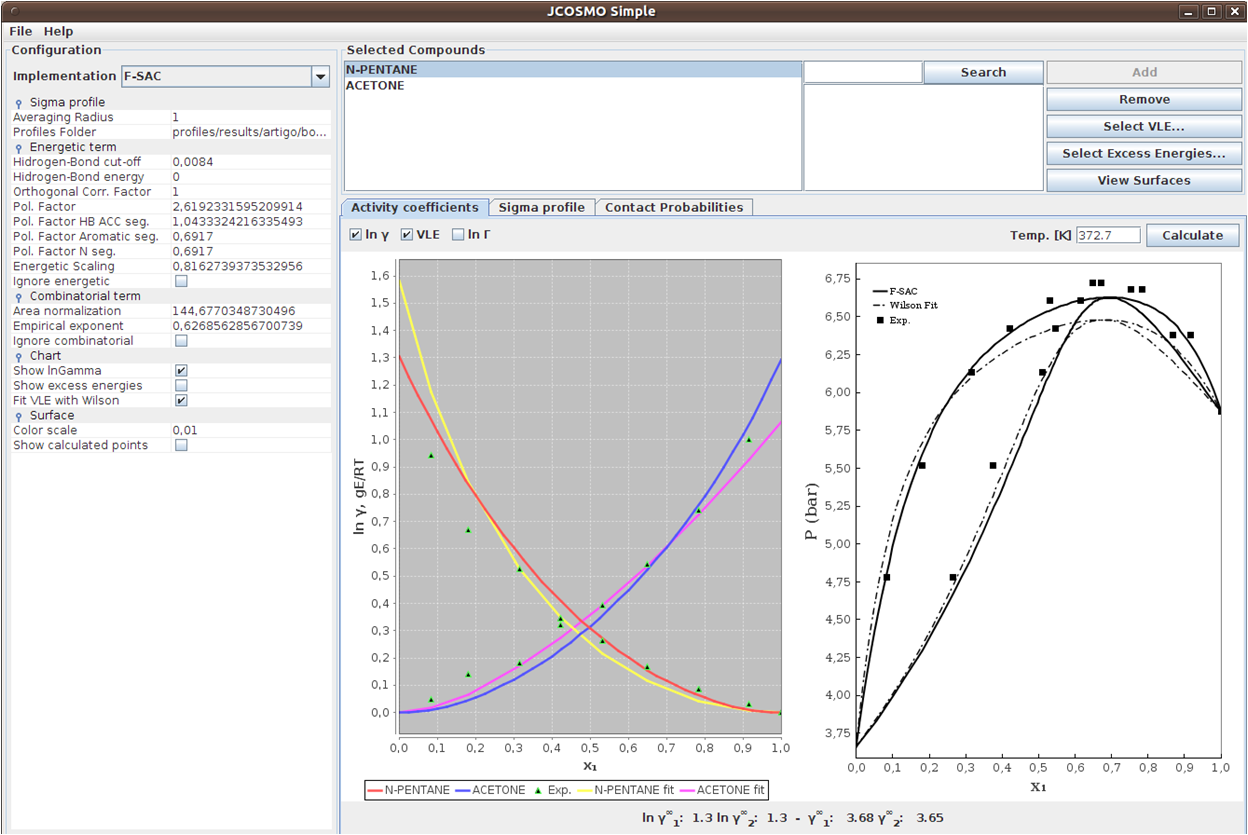
\includegraphics[width=1\textwidth]{img/jcosmo1}
		\end{center}
	
		\column{.3\textwidth}
		\begin{center}
			
\includegraphics[width=1\textwidth]{img/jcosmo_qr}
		\end{center}
	\end{columns}
\end{frame}

\begin{frame}
  \frametitle{Programa JCOSMO: Visualização das superfícies}
	\begin{columns}[t]
		\column{.6\textwidth}
		\begin{center}
			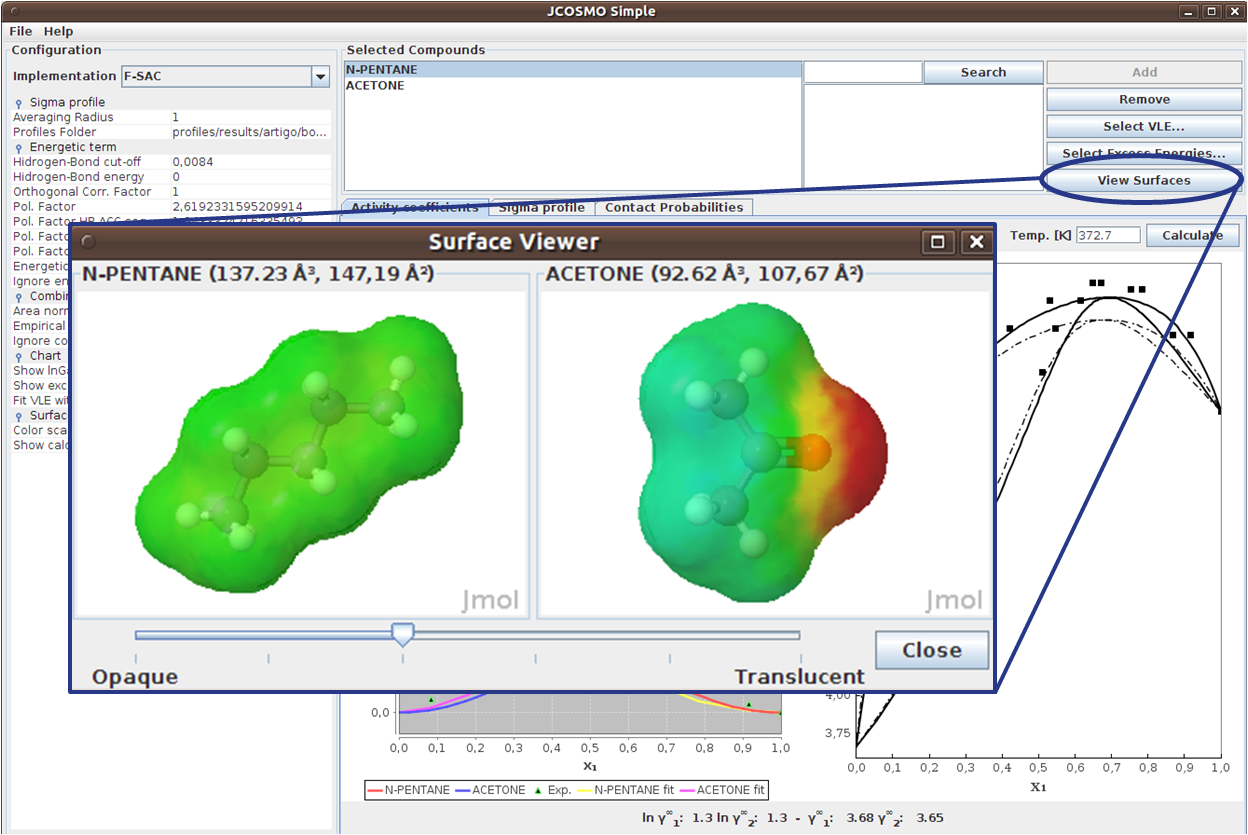
\includegraphics[width=1\textwidth]{img/jcosmo2}
		\end{center}
	
		\column{.3\textwidth}
		\begin{center}
			
\includegraphics[width=1\textwidth]{img/jcosmo_qr}
		\end{center}
	\end{columns}
\end{frame}


\subsection{F-SAC}
\begin{frame}[plain]
  \frametitle{Novo modelo F-SAC: Motivação}
  \begin{itemize} 
    \item Embora os modelos COSMO-RS contenham características teóricas excepcionais,
    	em geral os resultados obtidos podem ser considerados de qualidade semi-quantitativa
    \item Boa precisão normalmente é obtida através de modificações empíricas.
  \end{itemize}
  \begin{center}
  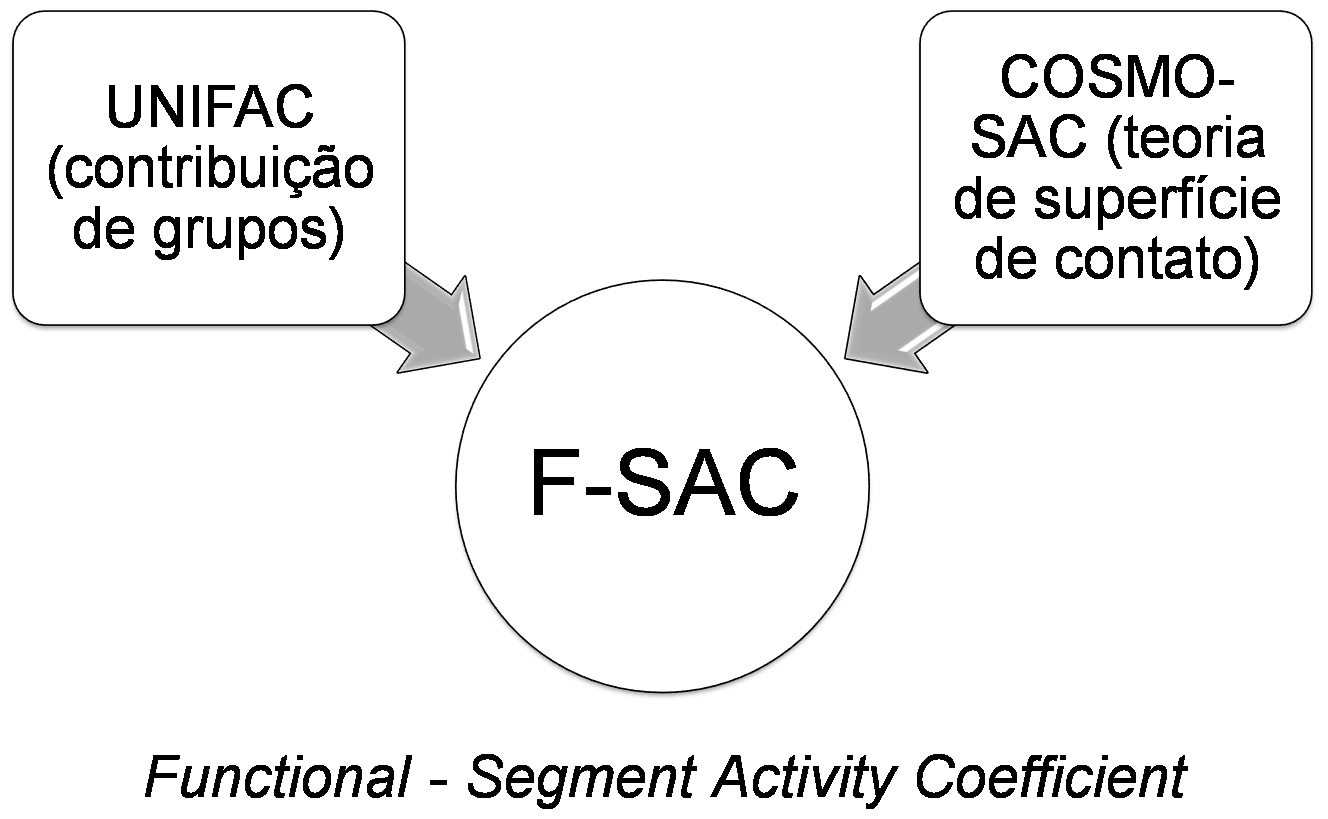
\includegraphics[width=0.55\textwidth]{img/fsac}
  \end{center}
\end{frame}

\begin{frame}
\frametitle{Diferença entre COSMO-SAC e F-SAC}
\begin{columns}[c]
\column{.6\textwidth}
\begin{center}
  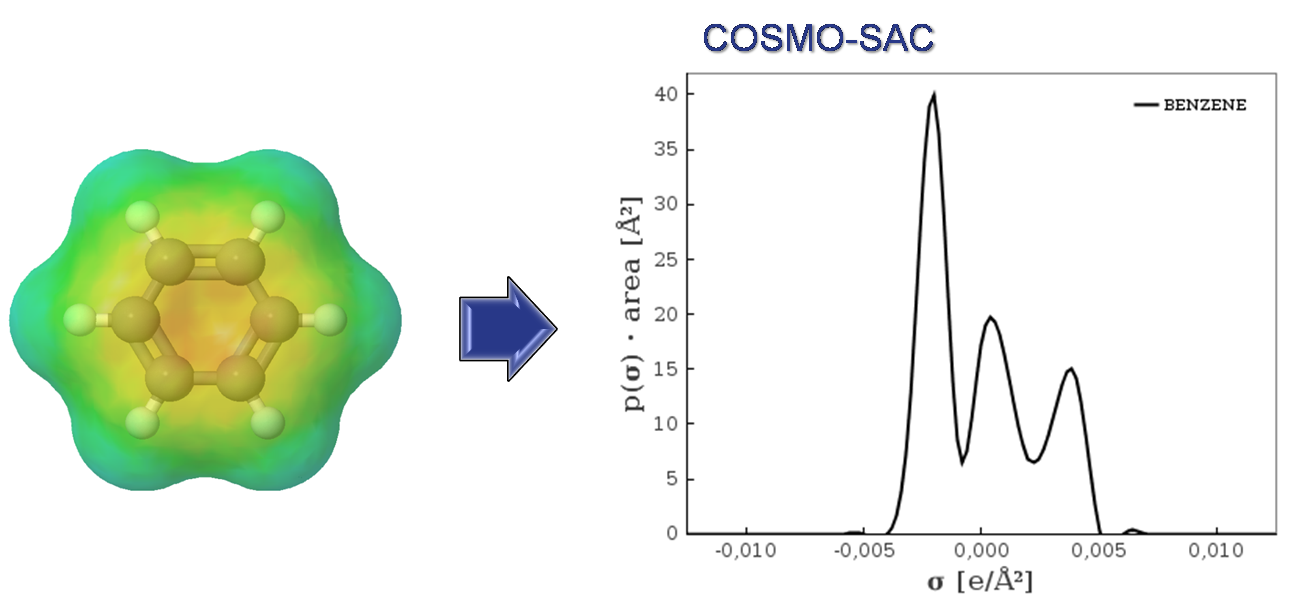
\includegraphics[width=0.75\textwidth]{img/perfil1}\\
  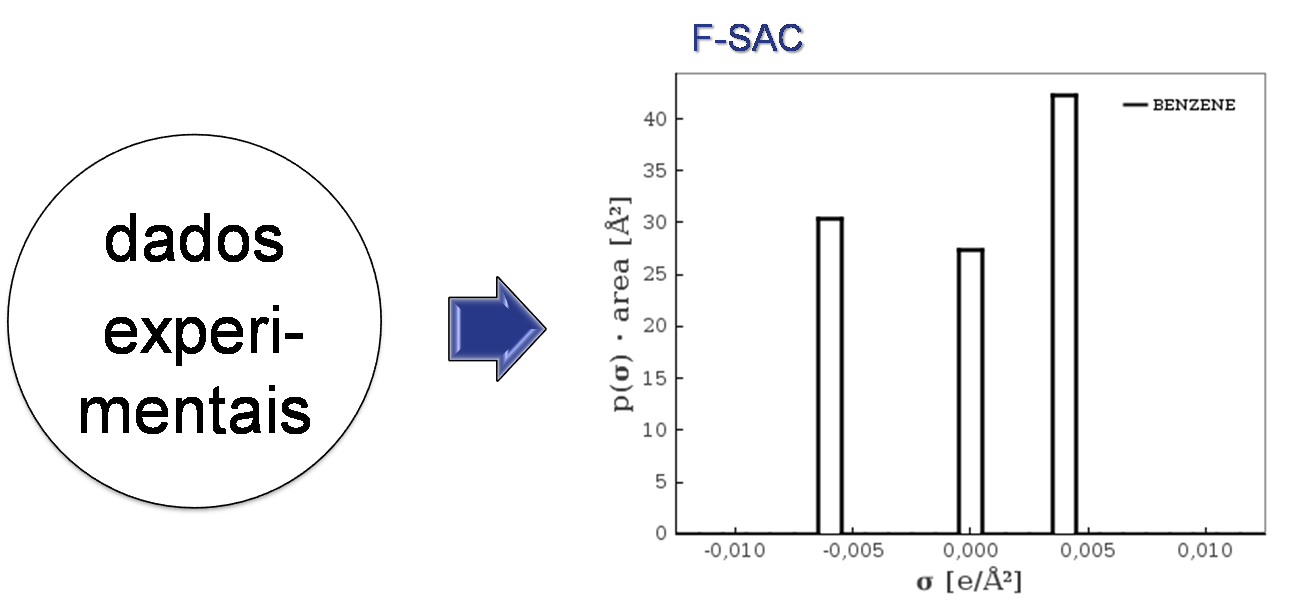
\includegraphics[width=0.75\textwidth]{img/perfil2}
\end{center}
\column{.5\textwidth}
\pause
\begin{itemize}
  	\item O equacionamento dos modelos é idêntico, a diferença
  		está no perfil sigma
    % \item Área superficial dos grupos é idêntica
    \item No F-SAC há uma fração da área neutra
    	outras duas frações com cargas
\end{itemize}
\end{columns}
\end{frame}

\begin{frame}
  \frametitle{Representação do perfil sigma}
  \begin{description}
	\item [$p_i(\sigma)$] $= \sum_k{\nu_k^{(i)}p_k(\sigma)}$
 	\end{description}
  \begin{center}
  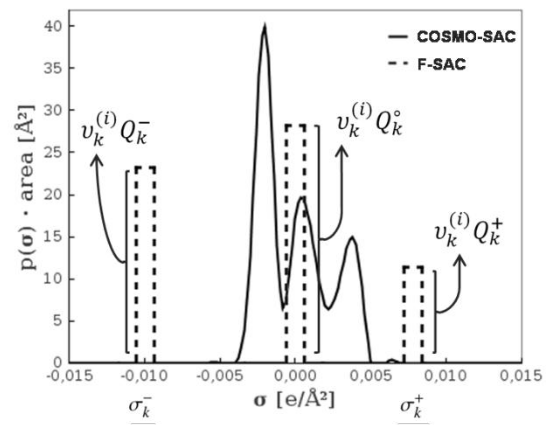
\includegraphics[width=0.45\textwidth]{img/perfil_fsac}
  \end{center}
\end{frame}

\begin{frame}
  \frametitle{Parâmetros do modelo}
  \begin{itemize}
    \item Parâmetros a serem calibrados com base em dados experimentais,
    	para cada grupo funcional $k$:
	\begin{description}
	\item [$Q_k$] área total do grupo, valor inicial é determinado com base em cálculos
		COSMO
	\item [$Q_k^+$] área do grupo funcional com carga positiva
	\item [$Q_k^-$] área do grupo funcional com carga negativa
	\item [$\sigma_k^+$] densidade de carga do segmento positivo
 	\end{description}
    \item Outros parâmetros determinados:
	\begin{description}
	\item [$Q_k^\circ$]  $= Q_k - Q_k^+ - Q_k^-$ é a área neutra do grupo
	\item [$\sigma_k^-$] $= \sigma_k^+Q_k^+ / Q_k^-$ é densidade de carga do segmento negativo
 	\end{description}
  \end{itemize}
\end{frame}

\begin{frame}
  \frametitle{Recomendaçõs para definir grupos funcionais}
  \begin{enumerate}
    \item A geometria do grupo funcional (ou seja, ângulo de ligação, etc.)
    deve ser a mesma independente da molécula em que o grupo ocorra.
    \item Cada átomo no grupo funcional deve ter aproximadamente a mesma
    carga em todas as moléculas em que o grupo ocorra, e o \textbf{grupo deve
    ser aproximadamente neutro}.
    \item Cada grupo funcional deve ser a menor entidade que a molécula pode
    ser dividida em uma coleção de grupos neutros.    
  \end{enumerate}
\end{frame}

\begin{frame}[plain]
  \frametitle{Seleção dos grupos: exemplo do grupo cetona}
  \begin{itemize}
    \item O centro do grupo funcional deve ser localizado, \ce{C=O}.
    \item O grupo é expandido a partir do seu centro para abranger uma
    \textbf{área neutra} da molécula.
    \item Por exemplo, \ce{CH3COCH3} para acetona, \ce{CH2COCH2} para dibutil
    cetona e \ce{CH3COCH} para metil isopropil cetona.
  \end{itemize}
  \begin{center}
  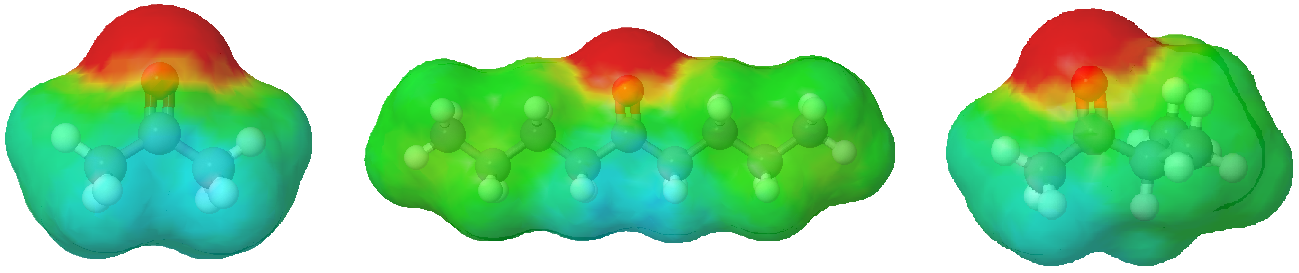
\includegraphics[width=0.9\textwidth]{img/cetona}
  \end{center}
  \begin{itemize} \pause
  \item Para que o número de parâmetros não aumente muito,
  	é assumido que todos os \textbf{subgrupos} acima pertencem a um \textbf{mesmo grupo}
  	com os mesmos parâmetros $Q_k^+$, $Q_k^-$ e $\sigma_k^+$, diferindo apenas na área
  	e volume total.
  \end{itemize}
\end{frame}

\begin{frame}
  \frametitle{Necessidade de novos grupos: moléculas complexas}
  \begin{itemize}
    \item Dois ou mais heteroátomos estão muito próximos.
    \item A interação entre os átomos não é descrita adequadamente pela simples
    soma dos grupos.
    \item É preciso definir novos grupos, menos abrangentes.
  \end{itemize}
  \begin{center}
  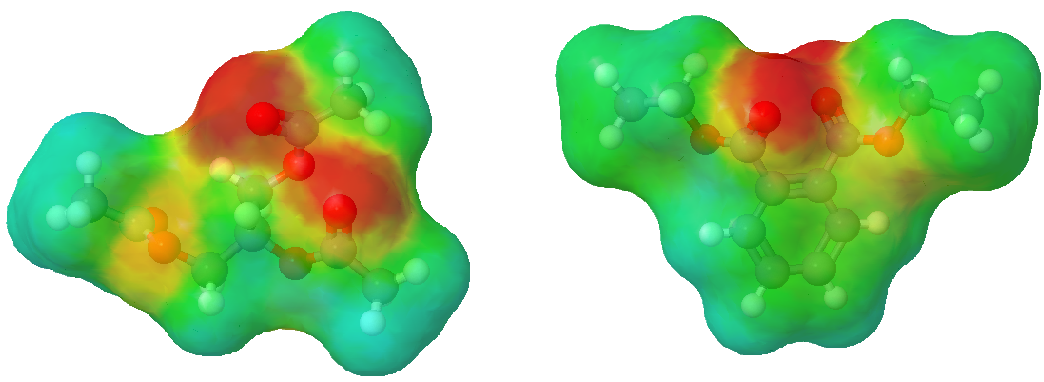
\includegraphics[width=0.6\textwidth]{img/ester_1}
  \end{center}
  \begin{footnotesize}
  É o caso da \textbf{triacetina} e do \textbf{dietil ftalato}
  \end{footnotesize}
\end{frame}

\begin{frame}
  \frametitle{Necessidade de novos grupos: geometrias diferentes}
  \begin{itemize}
    \item A geometria do grupo funcional deve ser a mesma, independente da
    molécula em que este grupo ocorra
    \item Éster cíclico tem diferentes ângulos de ligação quando comparado com
    um linear
  \end{itemize}
  \begin{center}
  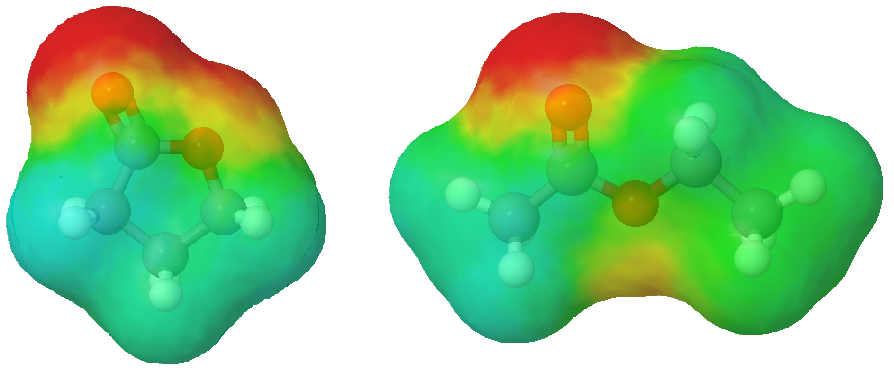
\includegraphics[width=0.6\textwidth]{img/ester_2}
  \end{center}
  \begin{footnotesize}
  Um novo grupo foi adicionado para a \textbf{$\gamma$-Butirolactona}.
  \end{footnotesize}
\end{frame}

\section{Conclusão} 

\begin{frame}
  \frametitle{Equações de Estado}

  \begin{itemize}
    \item As Equações de Estado são utilizados basicamente quando possuem
   	equilibrio de fase em alta pressão com pouco desvio da idealidade:
    \begin{itemize}
      \item Troca térmica
      \item Equilíbrio de fases
      \item \ldots
    \end{itemize}
    \end{itemize}
\end{frame}

\begin{frame}
  \frametitle{Modelos de $\gamma$}

  \begin{itemize}
    \item Os modelos de $\gamma$ são utilizados basicamente quando possuem
   	equilibrio de fase em baixas pressões
    \begin{itemize}
      \item Coluna de destilação
      \item Flash
    \end{itemize}
    \end{itemize}
\end{frame}

\begin{frame}
  \frametitle{Equações de Estado + Modelos de $\gamma$}
  \begin{itemize}
    \item As Equações de Estado acopladas a modelos de $\gamma$ são utilizados
    basicamente quando possuem equilibrio de fase em alta pressão com alto
    desvio da idealidade:
    \begin{itemize}
      \item Troca térmica
      \item Equilíbrio de fases
       \item Coluna de destilação
      \item Flash
      \item \ldots
    \end{itemize}
    \end{itemize}

\end{frame}

\begin{frame}
\Huge{\centerline{Obrigado}}
\end{frame}

\end{document} 
